\documentclass[12pt]{article}
\usepackage{hyperref}
\usepackage{authblk}
\usepackage{graphicx}
\usepackage{amsmath}
\usepackage{amssymb}
\usepackage{enumitem}
\usepackage{amsfonts}
\usepackage{array}
\usepackage{xcolor}
\usepackage{tikz}
\usepackage{pifont}
\usepackage{fontawesome5}
\usepackage{tikz-3dplot}
\usepackage{forest}
\usepackage{cancel}
\usepackage{ulem}
\usepackage{subcaption}
\usepackage{booktabs}
\usepackage{placeins}
\usepackage{float}
\usepackage[margin=1in]{geometry}
\floatplacement{figure}{H}
\title{Forecasting Grocery Store Product Sales}
\author{Austin Lackey}
\author{Tomy Sabalo Farias}
\author{Sam Herold}
\affil{DSCI 478, Colorado State University}


\begin{document}
\maketitle
% GitHub link
\begin{center}
    \href{https://github.com/austinlackey/store-sales-forecasting}{\textbf{GitHub Repository}}
\end{center}

\begin{abstract}
This paper presents a methodology for forecasting grocery store sales across many stores and product subsets.
The data used in this project is from Favorita Grocery Stores in Ecuador from 2013 to 2017 and is provided by Kaggle.
A link to the data can be found in the references at the end of this paper. The work entailed individual, predictive models that were narrowed down to our best and final model.
In this project, we use a variety of models including linear \& polynomial regression, and gradient-boosting. 
Our methodology is split into two main sections: the characteristics surrounding the problem and our model solution. We will be centering our write-up around a gradient-boosting model that was most effective.
\end{abstract}

\section{Introduction}
\subsection{Background}
Time series data is data collected and marked by time. 
Because the sequence of the data is meaningful, there may be trends and patterns in time-series data that are different to traditional data.
Time is typically the main predictor variable, but we can cleverly add other features to increase our models accuracy\cite{timeseries}.
\\
\\
The Store Sales time series forecasting dataset contains sales data from Favorita Grocery Stores in Ecuador from 2013 to 2017\cite{kaggle}.
Sales data is broken down by store and product category for each day (1,782 pair-wise combinations $=stores \times products$).
\subsection{Problem Statement}
The goal of this project is to forecast sales for each store and product category combination one day into the future while reducing $RMSE$.
$RMSE$ is defined as the square root of the average of the squared differences between the forecasted and actual sales.
\[ RMSE = \sqrt{\frac{1}{n}\sum_{i=1}^{n}(y_i - \hat{y}_i)^2} \]
\subsection{Data}
\begin{table}[H]
\centering
\begin{tabular}{|c|c|c|p{7cm}|}
\hline
\textbf{Variable} & \textbf{Type} & \textbf{Unique Counts} & \textbf{Description} \\ \hline
date & datetime64 & 1684 & Date-stamp of the sales data \\ \hline
store\_nbr & int64 & 54 & Store number \\ \hline
family & categorical & 33 & Product family/category (Grocery, Beverages, Deli, etc.) \\ \hline
city & categorical & 22 & City of the store \\ \hline
state & categorical & 16 & State of the store \\ \hline
type & categorical & 5 & Type of store (A, B, C, D, E) \\ \hline
cluster & int64 & 17 & Cluster of the store (Similar stores grouped together) \\ \hline
promotion & int64 & 2 & Product Promotion (0 or 1) \\ \hline
oil\_price & float64 & decimal & Oil price for the day \\ \hline
\end{tabular}
\caption{Variable Descriptions}
\end{table}
For each day, we are making predictions for each store and product category combination (1,782 pair-wise combinations).
This is a challenging problem since sales are influenced by more than just the seasonality.
Below is an example that shows the sales over the course of a three-month period for only the top 5 product categories for the store with the most sales.
\\
\\
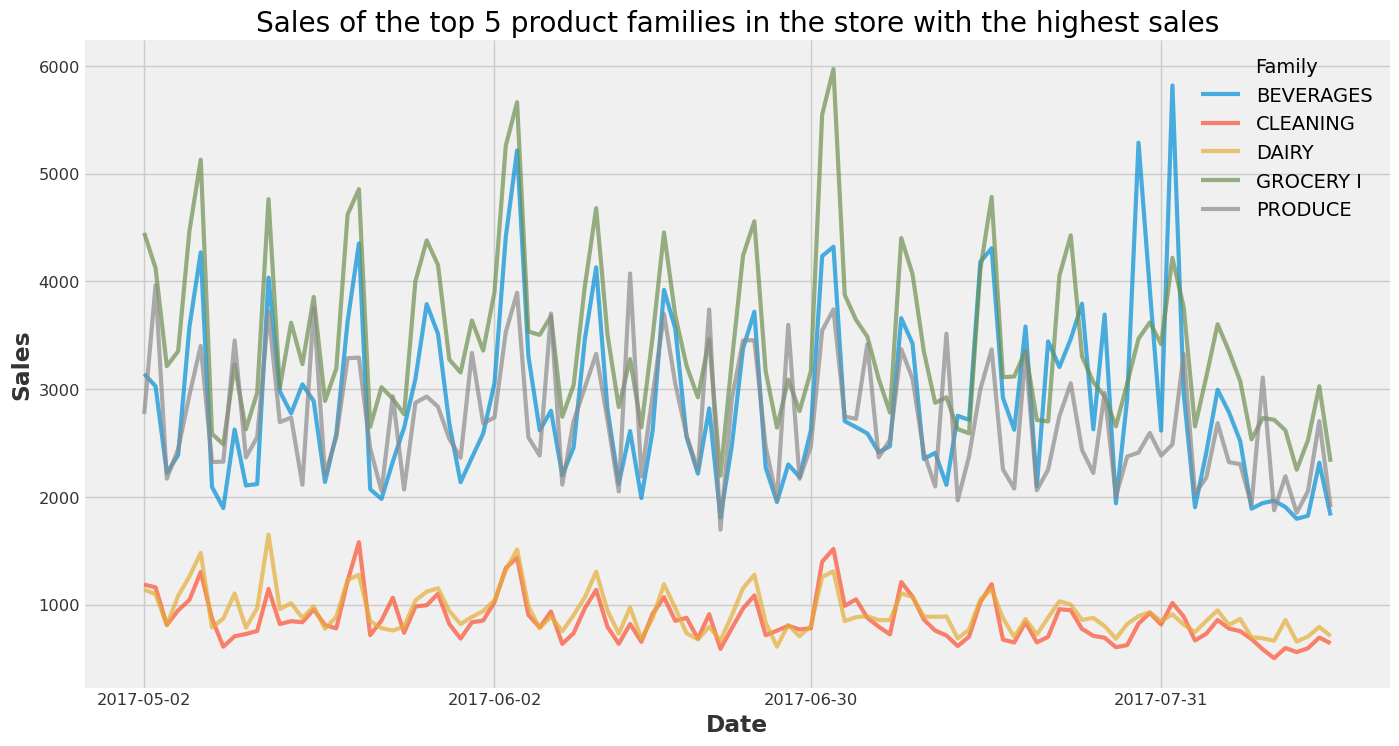
\includegraphics[width=\textwidth]{figures/Top 5 Products.png}
\captionof{figure}{Top 5 Product Categories for Store 44}
\begin{table}[H]
\centering
\begin{tabular}{|c|c|c|}
\hline
\textbf{Date} & \textbf{Store Number} & \textbf{Product Category} \\ \hline
2013-01-01 & 1 & Grocery \\ \hline
2013-01-01 & 1 & Beverages \\ \hline
2013-01-01 & 1 & Deli \\ \hline
\vdots & \vdots & \vdots \\ \hline
2013-01-01 & 54 & Grocery \\ \hline
2013-01-01 & 54 & Beverages \\ \hline
2013-01-01 & 54 & Deli \\ \hline
\vdots & \vdots & \vdots \\ \hline
2013-01-02 & 1 & Grocery \\ \hline
\vdots & \vdots & \vdots \\ \hline
\end{tabular}
\caption{Example of Pair-Wise Combinations}
\end{table}
\section{Solution}
\subsection{Feature Engineering}
The biggest challenge in this project was to create a feature set that would allow us to forecast sales for each store and product category.
Accurately predicting price based on date alone would is near impossible.
It is necessary to add more predictive features.
We found that the most important part in reducing $RMSE$ was to create a feature set that captured as much information regarding seasonality and trends as possible.
We created a feature set that included the following extra variables:

\begin{itemize}
    \item \textbf{Datetime Features:} We created features that captured what day of the week it was, the day of the month, the month, the quarter, the week of the year and the year. It is clear that the day of the week, and month, etc. can have some correlation with sales. As you can see in Figure 2 below, there is a clear seasonality in the data.
    \item \textbf{Lag Features:} A lag feature gives the model information about the previous day or days. We implemented a 7-day lag feature with the sales of previous days. It makes sense that the sales of yesterday or two days ago would have some kind of indication on the sales of today. This is common practice in time-series forecasting. Lag features essentially give the model more context and significantly increases accuracy.
    \item \textbf{Store-Specific Features:} We joined the store data with the sales data to give the model more information about the store. This includes information as specific as which product categories had a promotion that day.
    \item \textbf{Outside Data:} We also joined the sales data with oil prices since Ecuador is heavily dependent on the oil industry\cite{kaggle}. We can see that there is a negative correlation between oil prices and the sum of sales for stores within Ecuador in Figure 3 below.
\end{itemize}
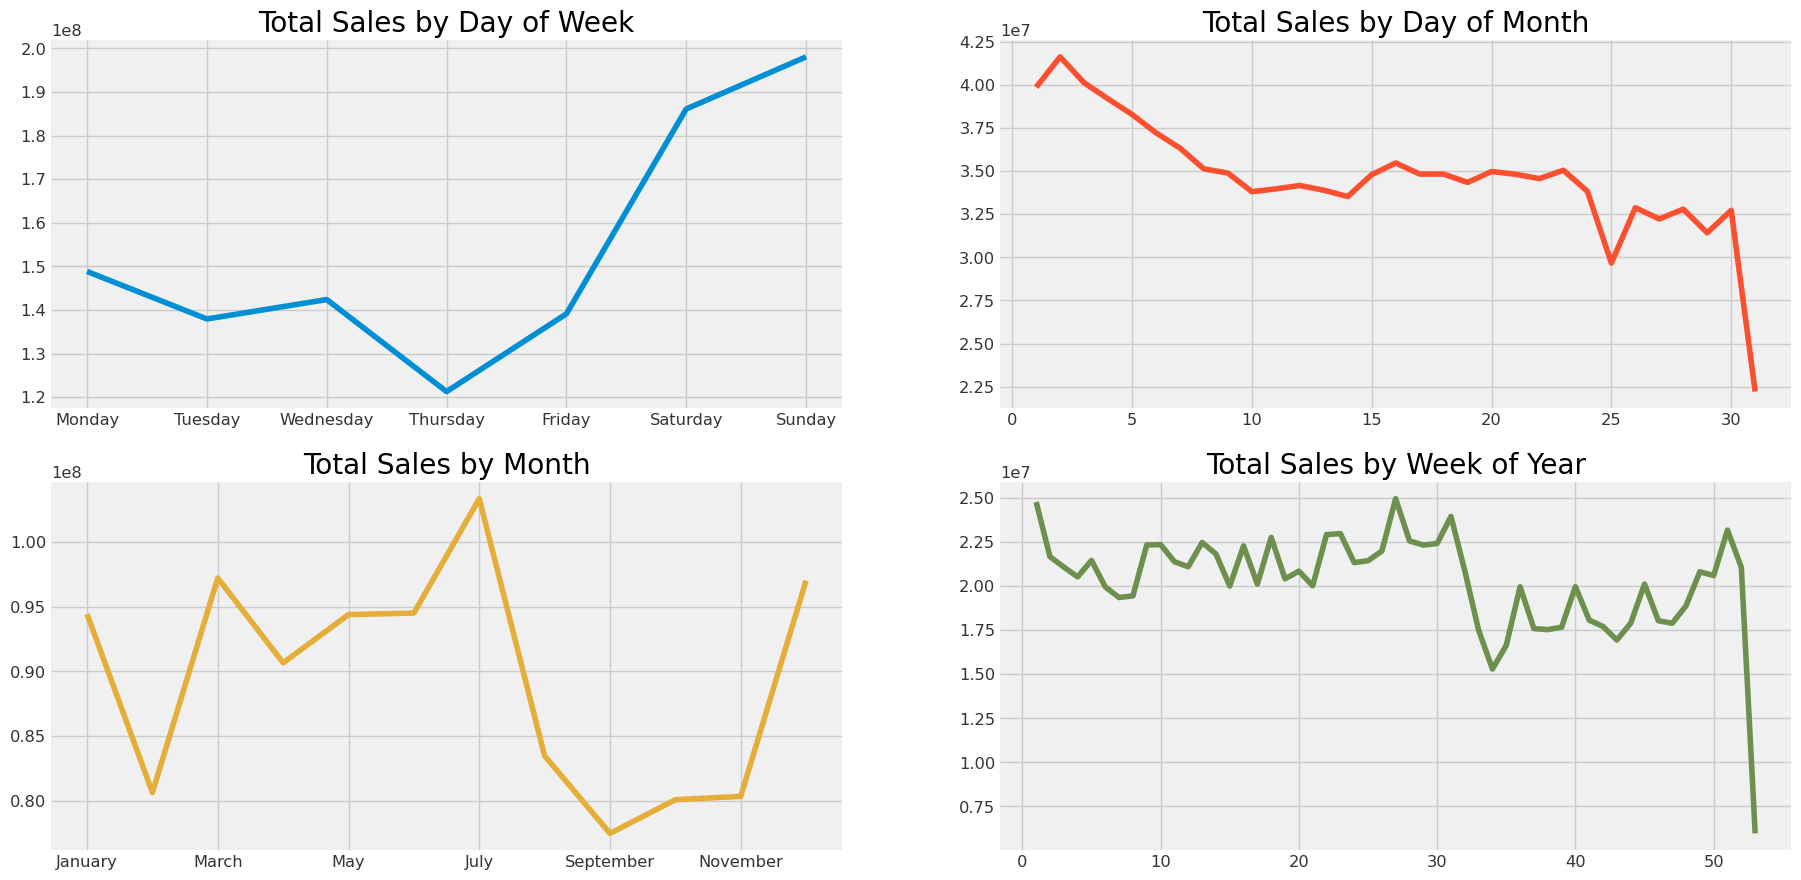
\includegraphics[width=\textwidth]{figures/seasonality.png}
\captionof{figure}{Seasonality}
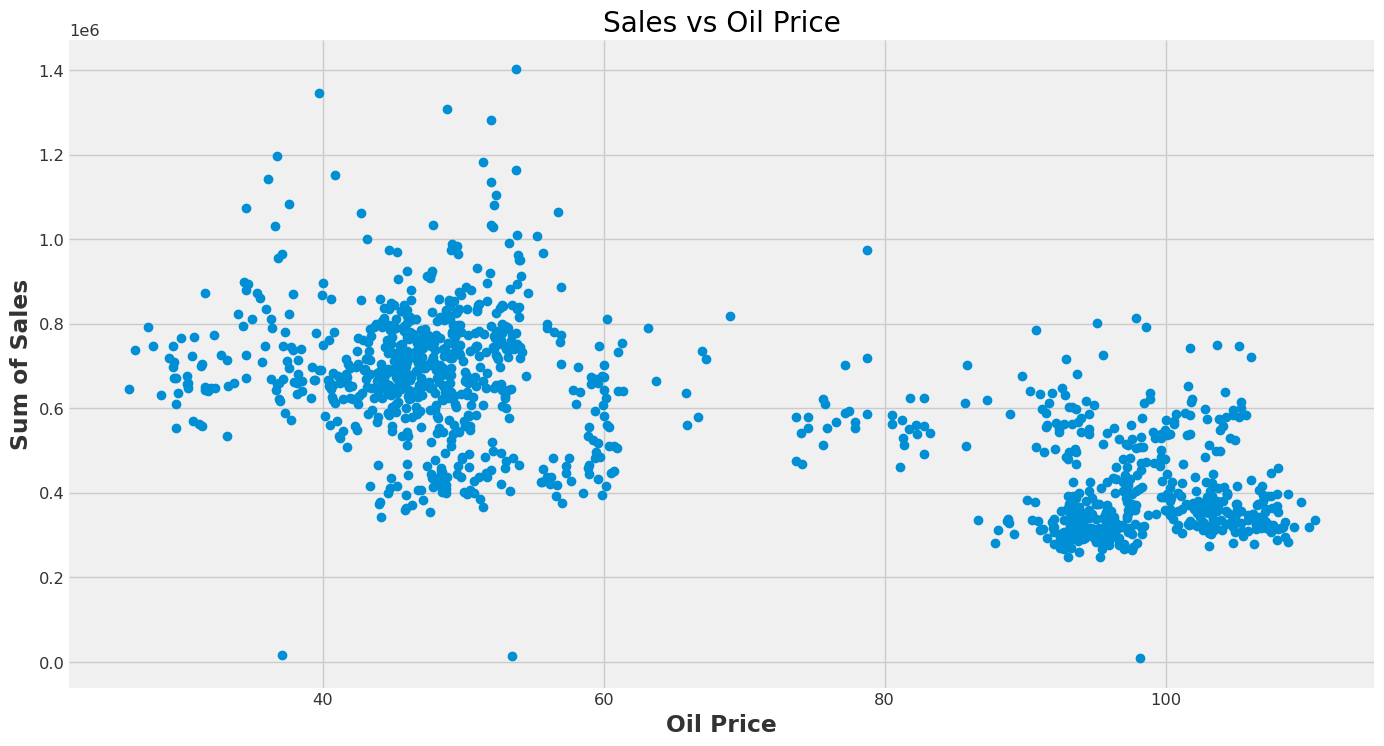
\includegraphics[width=\textwidth]{figures/oil.png}
\captionof{figure}{Oil Prices}

\subsection{Model Engineering}
\subsubsection{XGBoost Model}
Although we tested multiple models including linear and polynomial regression, we found that the best model for this problem was gradient boosting.
XGBoost is an open-source library that implements gradient boosting in an optimized way that makes it easy for data scientists to fine-tune their models\cite{xgboostInfo}.
The idea is that we are building a sequence of trees that are trained to minimize a cost function.
As mentioned in the previous section, we used $RMSE$ as our cost function, which is a very common metric for regression problems.
We set our model up with the following parameters:
\begin{table}[H]
\centering
\begin{tabular}{|c|c|}
\hline
\textbf{Parameter} & \textbf{Value} \\ \hline
base\_score & 0.5 \\ \hline
booster & gbtree \\ \hline
n\_estimators & 1000 \\ \hline
objective & reg:squarederror \\ \hline
max\_depth & 15 \\ \hline
learning\_rate & 0.1 \\ \hline
\end{tabular}
\caption{Variable Descriptions}
\end{table}
The base score is the initial prediction score for all instances, which is set to 0.5 by default\cite{xgboostDocs}.
We used the gradient boosting tree model with 1000 estimators(trees), although later in training a smaller number of estimators was found to be sufficient.
We used a max tree depth of 15 and a learning rate of 0.1.
Increasing the tree depth helps the model capture more complex patterns, however it can increase the risk of over-fitting\cite{xgboostDocs}.
In our case, we found that a tree depth of no more than 15 prevented over-fitting while maximizing the model's ability.

\subsubsection{Training the XGBoost Model}
After 114 iterations, our $RMSE$ converged to 319, which means that 114 estimators were enough to minimize the cost function.
We can see this in the plot and table below, after 100 iterations, the $RMSE$ begins to yield diminishing returns.
\begin{table}[H]
\centering
\begin{tabular}{|c|c|}
\hline
\textbf{Iterations} & \textbf{RMSE} \\ \hline
0 & 1326.11 \\ \hline
100 & 319.14 \\ \hline
114 & 319.10 \\ \hline
\end{tabular}
\caption{Iterations and RMSE}
\end{table}
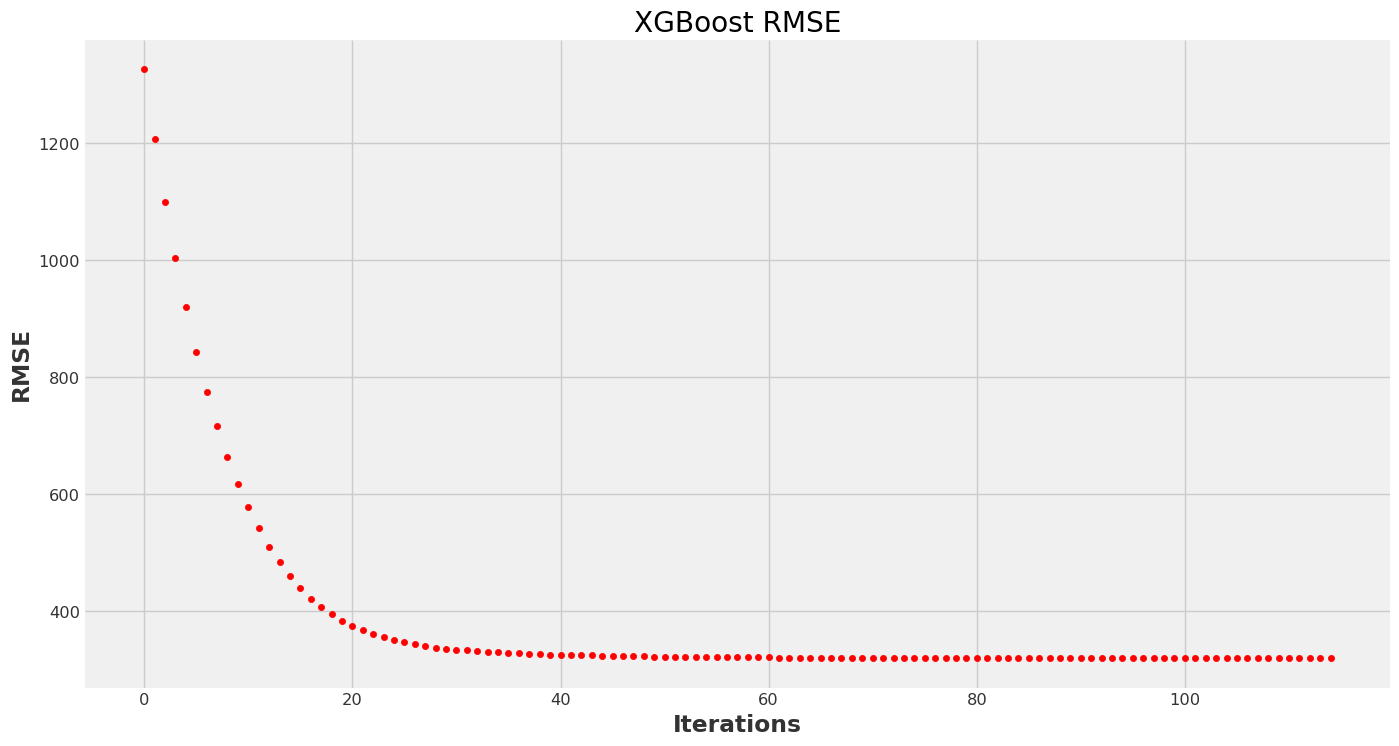
\includegraphics[width=\textwidth]{figures/rmse.png}
\subsubsection{Evaluating the Predictions}
The blue line in the plot below represents the actual sales, while the red line represents the predicted sales. Predictions were made from 2016-12-05 to 2017-08-15 which accounted for 15\% of the data, RMSE for all stores and products over this time period was 319.10.
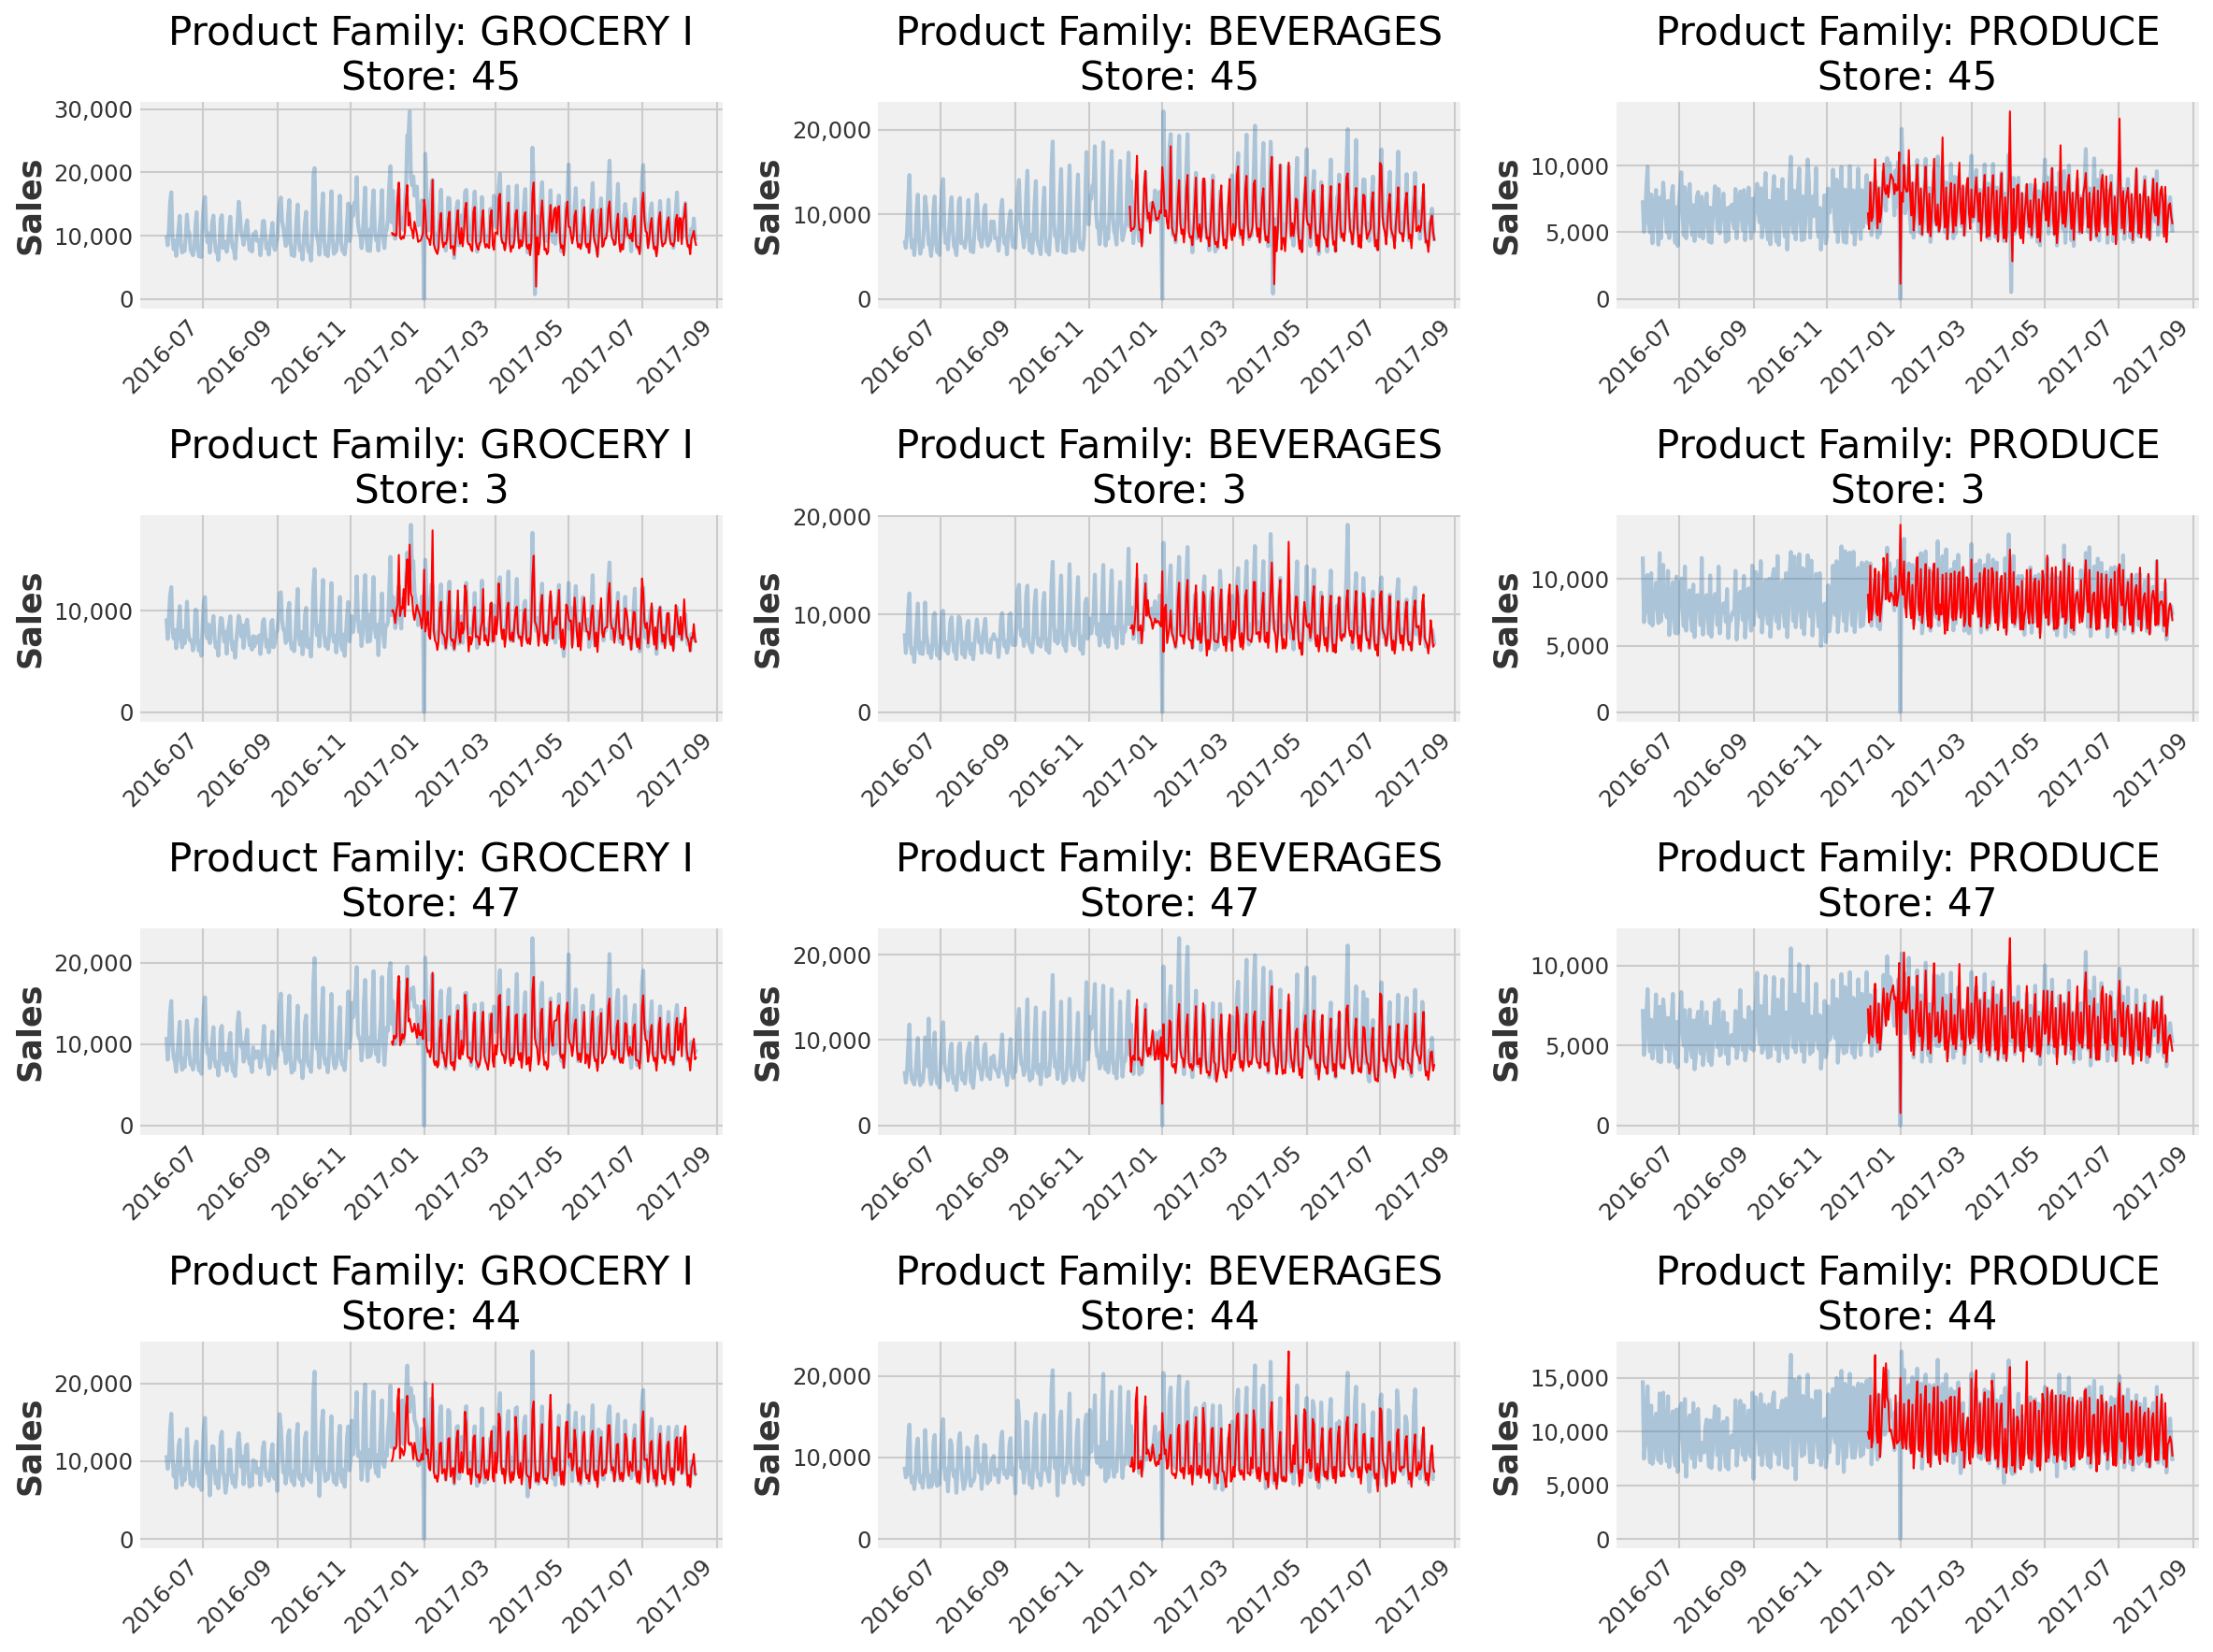
\includegraphics[width=\textwidth]{figures/XGBoost.png}
\captionof{figure}{XGBoost Predictions}
Since we are making 1,782 pair-wise predictions, let's just take a look at the top 3 product categories for the top 4 stores.
More specifically, lets look at how the predictions compare to the actual sales for stores 3, 44, 45, and 47 in the top 3 product categories, Grocery I, Beverages and Produce.
Our model does a decent job at capturing the the seasonality and trends in the data. 
There are certain product categories it does better, but overall the model is able to capture a lot of variation when it comes to different stores and product categories.
\section{Conclusion}
In this project, we were able to forecast sales for each store and product category using the XGBoost model.
We found that the most important part in reducing $RMSE$ was to create a vast feature set that captured as much information regarding seasonality and trends as possible.
This meant creating features that were specific to the stores, calendar features, lag and outside data such as oil prices.
If we were to improve this model, we would look into capturing holidays and other events that could influence sales.
It would also be interesting to see how the model performs with new LSTM models that have been recently developed.
\begin{thebibliography}{9}
\bibitem{timeseries}
Time Series Kaggle Course. Kaggle. Retrieved from \url{https://www.kaggle.com/learn/time-series}
\bibitem{kaggle}
Favorita Grocery Store Sales - Time Series Forecasting. Kaggle. Retrieved from \url{https://www.kaggle.com/competitions/store-sales-time-series-forecasting/data}
\bibitem{xgboostInfo}
XGBoost: A Complete Guide to Fine-Tune and Optimize your Model. Towards Data Science. Retrieved from \url{https://towardsdatascience.com/xgboost-fine-tune-and-optimize-your-model-23d996fab663}
\bibitem{xgboostDocs}
XGBoost Documentation. dmlc. Retrieved from \url{https://xgboost.readthedocs.io/en/stable/python/python_api.html}

\end{thebibliography}
\end{document}